\documentclass[11pt]{article}
\usepackage[margin=1in]{geometry}
\usepackage{amsmath}
\usepackage[backend=biber,style=authoryear-comp,maxcitenames=2]{biblatex}
\usepackage{csquotes}
\usepackage{xcolor}
\usepackage{hyperref}
\usepackage{tikz}
\usepackage{framed}

% Add a bibliography file
\addbibresource{refs.bib}

\title{texMini Test Document}
\author{Test Author}
\date{\today}

\begin{document}

\maketitle

\section{Introduction}

This is a test document for texMini with bibliography support \cite{testwork2024}. Basic math: $a^2 + b^2 = c^2$

\section{Basic Math}

Inline math: $E = mc^2$ and $f(x) = x^2 + 1$.

Display math:
\begin{equation}
    \int_0^1 x^2 dx = \frac{1}{3}
\end{equation}

Matrix example:
\begin{equation}
    A = \begin{pmatrix}
        a_{11} & a_{12} & \cdots & a_{1n} \\
        a_{21} & a_{22} & \cdots & a_{2n} \\
        \vdots & \vdots & \ddots & \vdots \\
        a_{m1} & a_{m2} & \cdots & a_{mn}
    \end{pmatrix}
\end{equation}

\section{Lists}

\begin{itemize}
    \item First item
    \item Second item
    \item Third item
\end{itemize}

\begin{enumerate}
    \item Numbered item one
    \item Numbered item two
    \item Numbered item three
\end{enumerate}

\section{Colors and Hyperlinks}

texMini includes xcolor and hyperref:

\begin{itemize}
    \item \textcolor{red}{Red text}
    \item \textcolor{blue}{Blue text}
    \item \textcolor{green}{Green text}
    \item Link to \href{https://github.com/alexmill/texMini}{texMini repository}
\end{itemize}

\section{Graphics with TikZ}

texMini includes pgf/tikz for creating graphics:

\begin{center}
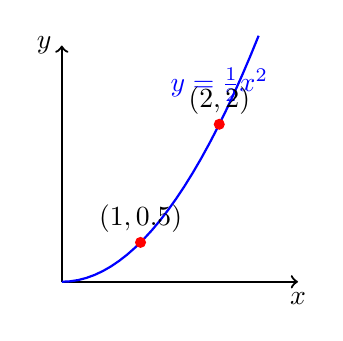
\begin{tikzpicture}
    % Draw a simple diagram
    \draw[thick, ->] (0,0) -- (3,0) node[anchor=north] {$x$};
    \draw[thick, ->] (0,0) -- (0,3) node[anchor=east] {$y$};
    
    % Draw a function
    \draw[blue, thick, domain=0:2.5] plot (\x, {0.5*\x*\x});
    \node[blue] at (2, 2.5) {$y = \frac{1}{2}x^2$};
    
    % Draw some points
    \fill[red] (1,0.5) circle (2pt);
    \fill[red] (2,2) circle (2pt);
    
    \node[anchor=south] at (1,0.5) {$(1,0.5)$};
    \node[anchor=south] at (2,2) {$(2,2)$};
\end{tikzpicture}
\end{center}

\section{Framed Content}

texMini includes the framed package:

\begin{framed}
This is content inside a frame. This tests that the framed package is working correctly with texMini.
\end{framed}

\section{Bibliography Test}

This document cites multiple works: \cite{testwork2024} and the classic \cite{knuth1984texbook}.

\section{Conclusion}

If this document compiles successfully with bibliography, then texMini's bibliography support is working correctly. The document should include:

\begin{itemize}
    \item Proper bibliography processing with biber
    \item Citation formatting with biblatex
    \item All essential packages (math, graphics, colors, etc.)
\end{itemize}

\printbibliography

\end{document}
